\documentclass[10pt]{article} 

%%%%%%%%%%%%%%%%%%%%%%%%%%%%%%%%%%%%%%%%%%%%%%%%%%%%%%%%%%%%%%%%%%%%%%%%%%

\usepackage{graphicx}
\usepackage[usenames,dvipsnames]{color}
\usepackage{cochineal}
%\usepackage{euler}
\usepackage[T1]{fontenc}


\usepackage[round]{natbib}
\bibliographystyle{myMBE}



%\bibliographystyle{plainnat}
\usepackage{fullpage} 
\usepackage{verbatim} 
\usepackage{color} 
\usepackage[colorlinks=true,linkcolor=Violet,citecolor=Violet,urlcolor=blue]{hyperref} 
\usepackage{listings}
 

\title{
  {\Huge\color{red}U}nrooted 
  {\Huge\color{red}Ph}ylogenetic 
  {\Huge\color{red}O}rthology
\\(Documentation)
} 
\author{Jesus A. Ballesteros}
\date{Apr 2016}

%%%%%%%%%%%%%%%%%%%%%%%%%%%%%%%%%%%%%%%%%%%%%%%%%%%%%%%%%%%%%%%%%%%%%%%%%%%
\begin{document}
\maketitle
\section{Quick recipe}
\begin{enumerate}
\item Rename each FASTA file to include the OTU of species name. Using
the provided script \texttt{minreID.py}:
  \begin{verbatim} 
minreID.py SequencesAA.fasta Species_Name \|
  \end{verbatim}
\item Concatenate all the renamed FASTA files into a single reference
file.
  \begin{verbatim} 
cat *_withid.FASTA > AllSeqs.faa
  \end{verbatim}
\item AllvsAll BLAST. Create a BLAST database of the reference FASTA
file and search this file against this recently created database using
the csv output format. The \texttt{blast\_helper.sh} script is
provided to facilitate and parallelize this procedure.
  \begin{verbatim} 
Blast_helper.sh -i AllSeqs.faa
  \end{verbatim}
\item Cluster similar sequences into homologous families. An
additional $e$ value threshold can be enforced at this stage as well
as a minimum taxa threshold to filter out clusters with not enough
taxonomic representation.
  \begin{verbatim} 
BlastResultsCluster.py -in blast_out.csv -d \| -e
1e-50 -m 5 -R AllSeqs.faa
  \end{verbatim}
\item Phylogenetic pipeline. Perform multiple sequence alignment, gap
masking, alignment sanitation and phylogenetic inference on the
clusters.
  \begin{verbatim} 
cd ClusteRs/ 
paMATRAX+.sh -f -c
  \end{verbatim}
\item Orthology assessment with UPhO. Run all the gene family gene
trees through UPhO.
  \begin{verbatim} 
UPho.py -in *.tre -m 5 -S 0.95 -ouT -iP -R../AllSeqs.faa
  \end{verbatim}
\end{enumerate}

\clearpage

\tableofcontents
\section{Introduction} UPhO identifies orthologous splits from
gene-family trees and thus, strictly speaking, the only required input
are Newick formated trees (gene phylogenies) that satisfy a leaf naming
convention (explained below). Nevertheless, in most cases gene-family
trees need to be estimated from a collection of anonymous genomic
sequences (draft genomes, gene models, EST, transcriptomes, etc.) from
a collection of taxa of interest.

The pipeline herein presented, describes a general approach to obtain
these gene trees from such type of input data, identify orthogroups and
analyze some of its basic properties. It incorporates common tasks in
bioinformatics for detecting sequence homology and estimate gene trees
that are not intrinsically part of UPhO. Decisions in all the steps
leading to the gene trees are let to the  judgment of the user. In this
documentation is presented a plausible choice in a much diverse
decision tree. If you use UPhO or any of its scripts, please cite the
the paper describing the method \citep{Ballesteros2016} and the respective 
third party programs used.

\section{Download \& install} All the scripts described in this
document are available at
\url{https://github.com/ballesterus/UPhO.git}. You can clone the
latest version using git or download the files directly from the
GitHub website.  The scripts provided can be executed as stand-alone
programs or their functions imported as python modules and called from
the Python interpreter.  To execute the scripts from any directory add
the folder containing the scripts to your PATH variable. Additionally,
add this same folder to the PYTHONPATH variable so the functions can
be imported by the Python interpreter.

Example: If the UPhO folder is cloned (copied) in the folder
\texttt{/home/UserName/}, add the following
lines to your \texttt{.bash\_profile}:
 
\begin{verbatim} 
export PATH="$PATH:/home/UserName/UPhO/" 
export PYTHONPATH="$PYTHONPATH:/home/UserName/UPhO/"
\end{verbatim}

Tip: For the changes to take effect without log off your current terminal session, run:\\
\texttt{source .bash\_profile}

\subsection{Dependencies} For orthology inference UPhO depends only of
Python 2.7.x with standard libraries and modules. Some other scripts,
such as \texttt{distOrth.py} and \texttt{Get\_FASTA\_from\_Ref.py} make use of ETE2
and/or Biopython modules.  Many of the steps for the workflow herein
exemplified consists of common tasks for which a wide variety of
programs are available including: gene homology, multiple sequence
alignment, gap masking, alignment sanitation, tree inference,
etc. Here we demonstrate a possible implementation of this pipeline
but in the end users should be able to modify these tools according to
the problem complexity or user preferences. For example, these scripts use
MAFFT aligner but MUSCLE \citep{Edgar04} or CLUSTAL-$\Omega$ \citep{Sievers539} could have been used for the same purpose.

Some of the tasks performed in the pipeline are computationally demanding 
and would benefit of running in a computer cluster. Specifically,
BLAST searches and the phylogenetic pipeline are the more demanding
and time consuming operations. The scripts provided for this operations
spread the task in many parallel processes but these can be further tuned
depending on the architecture and implementation. Talk to your cluster administrator
about options for running these computationally demanding task. 
Most of the other steps, including the orthology evaluation, 
could be run in reasonable times using standard computing resources (laptop).

Third party programs used in the workflow:

\begin{itemize}
\item{gnu-parallel} \citep{Tange2011}
\url{http://www.gnu.org/software/parallel/}
\item{mafft} \citep{Katoh2013}
\url{http://mafft.cbrc.jp/alignment/software/}
\item{MCL} \citep{vanDongen2000} \url{http://micans.org/mcl/index.html}
\item{NCBI-BLAST+} \citep{Camacho2009}
\url{http://blast.ncbi.nlcm.nih.gov/BLAST.cgi?PAGE_TYPE=BLASTDocs&DOC_TYPE=Download}
\item{trimAl} \citep{Capella-Gutierrez2009} \url{http://trimal.cgenomics.org}
\item{RAxML} \citep{Stamatakis2014}
\url{http://sco.h-its.org/exelixis/web/software/raxml/index.html}
\item{FastTree} \citep{Price2010}\url{http://meta.microbesonline.org/fasttree/}
\end{itemize}


Python modules:
\begin{itemize}
\item Biopython \citep{Cock2009}. This module is used by \texttt{Get\_fasta\_from\_Ref.py} to produce
FASTA files from lists of seqIDs. Tested with Biopython versions 1.63 and 1.66
\url{http:biopython.org}

\item ETE2 \citep{Huerta-Cepas2010}. This module is used in \texttt{distOrth.py} and
\texttt{disthOrth\_interactive.py} for mapping orthologs on a reference
tree. Tested with versions 2.2.1072 and 2.3.9
\url{http://etetoolkit.org/docs/2.3/}.
\end{itemize}


\section{Sequence and leaves identifiers}\label{sec:sequenceNames} For
correctly parsing, the sequence identifiers in FASTA files and the leaf
names in Newick tree files, should be composed of at least two fields;
the first being a species name consisting exclusively of alpha-numeric
characters and underscore (a-z, A-Z, 0-9, \_). The second field should
correspond to a unique sequence identifier, also composed of
alpha-numeric characters and underscore. Additional fields are
effectively ignored and therefore tolerated.

The fields must be separated by a custom character (default ``|'')
that is not in the set used for naming OTU's. Virtually any other
character could be used although common sense should prevent the use
of characters with special meanings in FASTA and Newick standards,
such as ``>'', ``:'', ``('', etc.

\textbf{Important}: The use of blank spaces and punctuation marks
(``.'' ``,'') should be avoided. These characters should be replaced or
removed from sequence identifiers for proper parsing.

The script \texttt{minreID.py} can assist with the renaming of each
file or the user can resort to stream line editors (awk, sed) to
comply with the naming requirements. This simple script takes as arguments the target file, species name to use and the custom delimiter.


Example:

\begin{verbatim} 
#Example of identifier in iput file assembly.fasta:
>c1212_g1_i2

minreID.py assembly.fasta mySpecies \|

#Example of renamed output file assemly_withids.fasta:
>mySpecies|000001c1212_g1_i2
\end{verbatim}

Note that the pipe character ``|'', which has a special meaning in
bash, must be scaped with ``\char`\\'' to be interpreted as a text character.

Tip: If seamless transition between aminoacid and nucleotide versions
are desired, original DNA sequences and their respective
translations can be renamed consecutively. The goal of this
procedure would be to obtain nucleotide (NT) and aminoacid (AA) FASTA
files where the name of their sequences is identical.  Before running
the renaming tool, verify that AA and NT files have the same amount of
sequences an that these are in the same order.  Files should be
inspected, verifying that such correspondence is correct.

\section{Grouping sequences into homologs} The first step towards
obtaining gene trees is grouping sequences into sets of homologous
genes. The task of clustering sequences into gene families is a
complex bioinformatic problem and an active area of research. Two
approaches are herein exemplified; one is based on explicit sequence
similarity thresholds, and another one is based on a natural
clustering strategy using the Markov clustering algorithm
\citep{vanDongen2000, Enright2002}. The starting point to any of these clustering approaches is
a text file with pairwise BLAST scores. To build this required
similarity table we used an all versus all BLAST strategy.

\subsection{All versus All BLAST} This is a very common bioinformatic
routine in which a database is created from one or many input FASTA
files, and then the same input file(s) is queried against the local
database. By doing so every single pairwise comparisons are computed.

To facilitate and in some degree accelerate these computations, a
shell script, \texttt{Blast\_helper.sh} is provided. The script
creates a local BLAST database and performs the search using
\texttt{blastp} with a relaxed e value trhreshold of $e = 1 \times
10^{-3}$. Alternatively searches can be done using \texttt{psiblast} using the flag \texttt{-p}. This script also invokes gnu-parallel to spread the queries
across as many processors as available in the system, This script
depends on a local version of BLAST+ (v2.2.x) and gnu-parallel.

The only required parameter for the \texttt{Blast\_ helper.sh} script is an input file (\texttt{-i}) in  FASTA format. This file normally contains the sequences of all the species of interest with the sequence identifiers in the format described above. Specific query files can be defined (\texttt{-q}). If no query file is provided the input file will be used as the query, thus performing a \emph{all vs. all BLAST} search.

Example:
\begin{verbatim}
#Create a database with ALL_Seq.fasta using as query sequences from
# ModelSpecies.fasta using psiblast.

blast_helper.sh -i All_Seq.fasta -q ModelSpecies.fasta -p
\end{verbatim}



Note: BLAST $e$ value is used here because of its commonality in
several bioinformatic applications, but the user should be aware of the properties  and limitations of this parameter.


\subsection{Get\_Fasta\_from\_Ref.py}\label{sec:getfastafromref} This
script is not part of the clustering procedure \emph{per se}. However, it is
called by other scripts in the pipeline to create FASTA format files
from a file containing list of FASTA identifiers and a ``reference''
FASTA file containing all the sequences of interest. Two inputs are
required by this script.
\begin{enumerate}
\item query (\texttt{-q}): A text file in which the identifiers of
the sequences to be written in a single file are listed on a single
line saparated \textbf{only} by commas ``,''.  Example query file:
\begin{verbatim} 
Species1,Species2,Species3
Species4,Species5,Species6,Species7
\end{verbatim}
\item Reference (\texttt{-R}: A FASTA file that contains at least all
the sequences listed in query. Sequence identifiers must be identical
in the query and the reference files. If a sequence in the query is not
found, the process will stop due to an error. Also, each sequence
identifier in the ``reference'' file must be unique or error would
prevent the execution.
\end{enumerate}

Custom output directory can be specified with the \texttt{-o} flag.
The files created are named using a prefix (\texttt{-p}) and
a unique sequential number. If specified or existing names are to be
used, the first element in each query line is identified by a
preceding ``\#''.
Example query file with explicit file names:
\begin{verbatim} 
#myFile1,Species1,Species2,Species3
#myFile2,Species4,Species5,Species6,Species7
\end{verbatim}

This last example, represents the basic output format to report a collections of 
sequences per line. This basic format is used for grouping homologous and orthologous sequences  alike. 

\subsection{Clustering}

\subsubsection{BlastResultsCluster.py (BRC)} This script process
the BLAST all vs all output file and creates a text file in which
sequence identifiers that form a cluster are listed one per
line. Additionally, the script allows the user to enforce a more
strict $e$ threshold as well as a minimum taxon representation. This
last condition, prevents clusters composed of only one, or less than a
minimum desidered number of species to be carried over for downstream
analyses. For orthology evaluation or phylogenomics, these cases are
either trivial or useless: e. g. orthogroup $A=\{SpA|seq1,
SpA|seq2,SpA|seq4, SpA|seq5\}$.

Identifying this undesirable gene clusters earlier in the pipeline
saves time and allows the computing efforts to be prioritized for
clusters likely to produced orthologs of interest.

A special case of homologs are those in which each sequence is derived
from a different species. Therefore, each sequences in this sets has no
match (within the specified parameters) with any other sequence from
the same species. Such instances represent putative single copy
genes. Nevertheless, users should be aware that sampling artifacts may
produce spurious sigle copy groups. This groups of single copy genes,
are trivial for orthology evaluation with UPhO.

Example: Consider the homolog-group: $B=\{SpA|seq1, SpB|seq2,
SpC|seq3,SpD|seq4\}$.  There is no way to falsify the assumption of
orthology because there is not evidence of a single gene duplication
event.

An option to find only these single copy homolo-groups is provided in
\texttt{BlastResultsCluster.py} using the flah \texttt{-sc}, see examples below. 
Most commoly,users would be interested in cases where more than one  homologs are present per species; the relation of these multiple genes 
are thus candidate to be inspected in the search of orthologs. The single
copy genes are nonetheless represented (a subset) of the collection
of homologs with species redundancy.


Examples:

Identify and group single copy sets with an additional $e$ value and at
least 4 taxa.

\begin{verbatim}
BlastResultsClusters.py -in BLAST_output.csv -e 1e-10
-m 4 -sc -R All.fasta
\end{verbatim}

Identify and group redundant set with same $e$ value and at least 4
taxa:

\begin{verbatim} 
BlastResultsClusters.py -in BLAST_output.csv -e 1e-10 -m 4 -R ALL.fasta
\end{verbatim}

For each run of BRC two clusters outputs are produced: (1) text file
with clusters based on the e value, and (2) text file with clusters
with equal or more than the minimum number of species.


Tip: The construction of FASTA files from the resulting clusters is
implemented in BRC. However, and to avoid producing large amount of
sequence files that may in the end not be analyzed, the user can run
various runs of BRC with a diverse combination of taxa and expectation
thresholds. The smaller text outputs of these runs can be inspected
and specific ones selected for downstream analyses. The FASTA files of
the homologs selected can be generated later with
\texttt{Get\_fasta\_from\_Ref.py}.

\subsubsection{MCL} The Markov clustering algorithm as implemented in
the program \texttt{MCL} is an alternative to the BLAST based clustering
strategy. The use of \texttt{MCL} for clustering proteins into cluster is
documented and exemplified in
\url{http://micans.org/mcl/index.html}. The starting point for \texttt{MCL}
procedure uses the same BLAST output already generated in the
previous step.


BlastResultsCluster.py can generate a formated ``abc'' file to use as
input for \texttt{MCL}.  An additional BLAST $e$ value can be applied similarly
as the one used with the pure BLAST clustering describe above. Other
parameters working on clusters (\texttt{-d -m -R}) are ignored when
the \texttt{-mcl} flag is present.

Example:
\begin{verbatim} 
BlastResultsCluster.py -e 1e-10 -mcl
\end{verbatim}

The user is refered to follow the instructions listed in the \texttt{MCL}
website for clustering proteins using the output provided by
BRC. Exploration of the parameters inflation parameter $i$ and
evaluation of there results are strongly suggested,

The resulting output of \texttt{MCL} is by default TAB delimited. This file can
be modified replacing TABS with ``,'' and the resulting file used as a
query for \texttt{Get\_fasta\_from\_Ref.py}

\begin{verbatim} 
sed 's/\t/,/g mcl mci40.out > mci40.csv'
\end{verbatim}

Tip: Removing clusters containing less than \emph{a priori} minimum
amount of taxa will save time in later stages of the pipeline. The \texttt{MCL}
program does not filter these cases but BRC can be invoked to perform
this last filering:

\begin{verbatim} 
#Process a csv MCLcluster file to retain only
#clusters with more 6 or more taxa

python -c 'import BlastResultsCluster as BRC; BRC.redundant("mcl_i14.csv", 6)'

\end{verbatim} 

The output of this procedure (\texttt{ClustR\_m6.txt}),
can be now used as a query for \texttt{Get\_fasta\_from\_Ref.py}

\section{Estimating gene trees phylogenies: \texttt{paMATRAX+.sh}}
This script is provided to facilitate and accelerate the estimation of 
gene trees from multiple unaligned sequence files. For each input file the following steps are performed:
Align $\rightarrow $Mask gap rich regions $\rightarrow$ Clean alignment
of short sequences $\rightarrow$ estimate a phylogenetic tree.  This
part of the pipeline is one of the most time consuming ones and its
complexity depends on a variety of factors, including, sequence
complexity, number of sequences in each file, etc. This shell script
uses GNU-parallel to each step of the phylogenetic pipeline in
parallel. First a multiple sequence aligner (MAFFT) is run on all the
sequences in the current directory with extension
\texttt{``.fasta''}. The resulting alignments are written to files
named as the input files, with extension \texttt{``.al''}, once this
process is finished (all files are aligned.) The alignments are
processed with triMAL to mask or remove ``gappy'' regions of the
alignment. The outputs of this steps are written to files with
extension \texttt{.fa}.

These trimmed alignments can be used for phylogenetic inference or be
processed with a custom script (\texttt{Al2Phylo.py}) for additional
cleaning procedure to inspect that, after the trimming, each
individual sequence has a minimum number of unambiguous
sites. Sequences failing this test are removed. This procedure
prevents that minimally overlapping sequences that after trimming end
up composed of only gaps or too few AA sites to be used in
phylogenetic inference. Finally the cleaning procedure, checks that
the number of taxa per alignment remains the same after cleaning; this
step avoids spending time and effort in analyzing homologs that would
not produce the orthologs with minimal taxonomic representation. the
output of the cleaning procedure are written in the same folder with
the suffix \texttt{``\_clean.fa''}. For example, assume we are
interested in finding orthologs present in at least six species and a
homolog-group has 20 sequences from eight species. After alignment,
trimming and cleaning, the number of sequences went down to 12 and
only five species are represented. Estimating a tree from this homolog
groups will be a waste of time and resources because there is no way
to obtain a six species ortho-groups from a five species gene family.

Phylogenetic inference can be performed using RAxML (default) or
FASTTREE (\texttt{-f}). Users should use their judgment based on the
number of alignments to process and their complexity to decide which
tool and parameters are best suited for their problem. The orthology
assessment depends heavily on the accuracy of gene tree but exhaustive
searches can be too time consuming to be completed on reasonable time,
especially if support values based on resampling are estimated.

To avoid repeating any step, \texttt{paMATRAX+.sh} automatically checks
if the corresponding  output file already exists in the current directory and skips
the input file if that is the case. For example, if after running the
pipeline on 1,500 sequence files a user discover that 5 alignments were not
processed by trimAl because this files contained stop codons. The user can replace the stop codons ``*'' by ``-'' in the five offending
\texttt{.al} files and run \texttt{paMATRAX+.sh} in the same working directory,
\texttt{paMATRAX+.sh} will not run MAFFT again because the
corresponding alignment files exist and will run trimAL and \texttt{RAxML} only on the
five missing files, because there are not corresponding trimmed files
(\texttt{.fa}) in the current directory.


Example using FastTree as tree estimator:

\begin{verbatim} 
#Move to the current directory where the unaligned homologs are located 
cd ClustRs/ 
paMATRAX+.sh -c -f

\end{verbatim}

Note: Typing \texttt{paMATRAX+.sh -h}, will print a short help screen
and the parameters and programs used in each step. The user can easily
modify this parameters by minimally editing the respective command
variables in the script. For example, some versions of fasttree source
produce a binary named ``FastTree'' or ``FastTreeMP''. Using
\texttt{paMATRAX+.sh} as it comes, would raise a flag indicating that
\texttt{``fastree: command not found''}. To fix this issue, the user can either rename
the binary to ``fasttree'' or edit the line number 25 of
\texttt{paMATRAX+.sh} in a text editor, changing
\texttt{fasttree\_cmd=``fasttree''} for
\texttt{fasttree\_cmd=``FastTree''}. The same commet applieds to
progarm specific parameter. If you use \texttt{paMATRAX+.sh} please
cite GNU-parallel and the corressponding programs used for each step.

\section{Orthology assessment with UPhO} Finally! you have trees of
several gene families and want to find the orthologs in these hundreds
of trees. The only input UPhO requires is a file or files with one or
more trees in Newick format. The only requirement for UPhO is that the leaves
are named following the naming convention explained in Section
\ref{sec:sequenceNames}. By default the field separator is the
character ``|''.  but custom delimiter can by defined with the flag \texttt{-d}. The
input files can be provided to UPhO using bash wildcards such as
\texttt{[]\{\}*?}. Example:

\begin{verbatim} 
#A single tree as input where field delimiter used in
#the leaves is the character @ 

UPhO.py -in myTre.tre -d @

# running UPhO on all the trees inside a directory named myTrees with
#extension ``.tre'' and where the leaves use the default delimiter.

UPhO.py -in myTrees/*.tre

\end{verbatim}

UPhO reports on the screen the number of orthogroups found per
tree. If in-paralogs are to be included with he orthogroups, the flag
\texttt{-iP} must be included. The minimum number of genes  per  orthogroups to
report is by default equal or greater than four but the user can modify
this threshold with the flag \texttt{-m}. Measures of topological
support (e.g. Bootstrap values) can be used as a criterion to discard
orthogroups derived from splits with low support. Users can define
specific support thresholds with \texttt{-S}. Any positive real number
(floating point) can be used for this parameter with the only assumption that greater
numbers represent better supported splits. The support evaluations is
applied universally to all orthology based evaluation, including those
that define in-paralogs.

Example:
\begin{verbatim} 
#Running UPhO accepting in-paralogs, incluiding atleast 12 species per
#orthogroup and derived from splits with at least 0.75 bootstraop
#support.

UPhO.py -m 12 -iP -S 0.75 -in *.tre

\end{verbatim}
 
Finally, users are more interested in comparing the actual orthologous sequences
or the trees derived from them. When the flag
\texttt{-ouT} is present the ortho-branches will be written to
individual files in Newick format and saved  in a folder named
\texttt{UPhO\_branches}.These trees can only be written during the
orthology evaluation phase; therefore, if the orthobranches of a previous run
are required, UPhO must be run again using the same parameters. If
orthobranches from multiple runs of UPhO want to be compared, the
Output folder must be renamed to avoid overwritting previous tree
files. The user should remember that these branches are derived from
the topolgy implied in the input gene-family tree and that phylogenetic 
re-ananlysis  of the orthologous sequences alone may differ from the
implied in the gene family tree.  In the same manner as with the
Homology section. Multiple sequences files can be written using the
flag \texttt{-R} pointing to a file with the sequeces of
interest. Again, this reference file should contain at least all the
sequences in the orthogroup and the sequences and leaf names should be
identical. These sequences are by default written to a folder named
\texttt{\char`\\UPhO\_sequences}.

Example:

\begin{verbatim} 
#A complex UPhO run combining a bash loop to obtain untrimmed aligned 
#FASTA files of each orthogroup. Notice that the
#firts part of the name in the aligned gene families and their trees
#is identical. The use of a single reference file will be problematic
#in this case because a given sequence may be present in more than one
#homolog alignment.

for i in *.tre 
do 
UPhO.py -m6 -iP -R ${i%_clean.*}.al -in $i -ouT 
cat UPhO_orthogroups.csv >> UPhO_allruns.csv 
done 
rm UPhO_orthogroups.csv

\end{verbatim}

Tip: To prevent writting large collections of sequences files, multiple
runs of UPhO can be evaluated withouth the \texttt{-R} flag. Each
UPhO\_orthogroups.csv file must be renamed between alternative runs to
prevent rewritting. If sequences are then required, they can be fetched 
using \texttt{Get\_fasta\_from\_Ref.py}

\section{Phylogenetic structure and congruence of orthologs} Simple
ways to evaluate the phylogenetic congruence of the orthologs can be
easily achieved. The ortho-branches themselves can be used to build a
species tree using super tree or compatibility methods, or to compute quartet networks.
 The procedures to do so will not  be explained in this document; however,  most of these methods require trees
 without taxon duplication. Tools for explicitly selecting a
particular representative leaf or sequence are already available. For
convenience, a function to do so over a file with one or many Newick trees
per line is included in \texttt{distOrth.py}, the resulting file with
only one sequence per species and with the leaf named using the
species name only are written to a file names \texttt{all\_ready.tre}.
Example:

\begin{verbatim} 
#Assuming the current folder contain only
ortho-branches, e. g. written to UPhO_branches/ 
cat *.tre > All.trees
python -c "import distOrth; distOrth.RemoveDupSpecies('All.trees')"

\end{verbatim}

\section{Distribution of orthologs with distOrth} A script
to map the distribution of orthologs across a give tree is included in
\texttt{distOrth.py} and its use is facilitated trough
\texttt{distOrth\_interactive.py}. These scripts leverage on the tree
annotation functionality of the ETE2 python module, a newer version of this 
module, ETE3 \citep{Huerta-Cepas2016}, has been recently released and is yet to be tested for compatibility.

There are two main input requirements for the mapping procedure:
\begin{enumerate}
  \item A species tree. This can be a tree estimated from the
orthologs or an external reference tree. The name of the leaves in
this tree must have at least all the species in the orthologs that are
gonna be mapped.
  \item A text file with the lists of orthologs and their sequence composition (\texttt{OG\_summary} hereafter). The  \texttt{UPhO\_orthogroups.csv} output or similar formated text file. An option is provided in \texttt{distOrth}  to create this file from a series of FASTA files.
\end{enumerate} 

\texttt{distOrth\_interactive.py} provides a series of options printed on the screen that guide the user to explore the distributions of the orthologs in the summary file. Most of these are self explanatory.


\begin{figure}[t!]
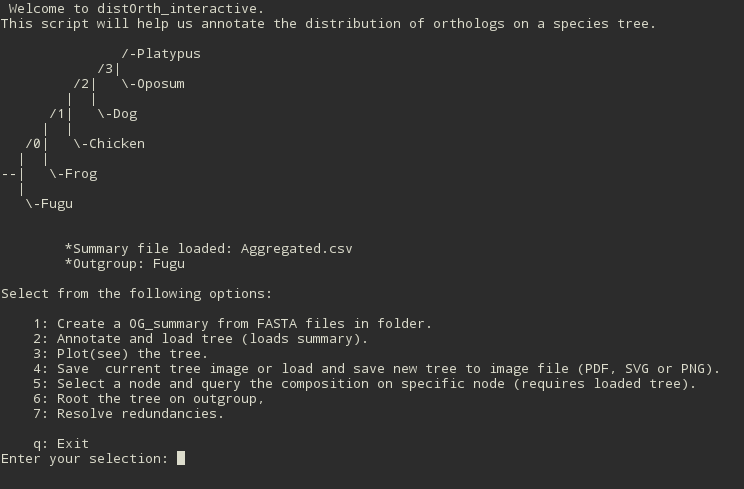
\includegraphics[width=\textwidth]{distOrthmenu}
\caption{Example of distOrth interactive showing the options available with a pre-loaded example tree.}
\end{figure}

\subsection{Create an \texttt{OG\_Summary.txt} from FASTA files}
One of the initial purposes of this script, was to be
able to compare orthogroups derived from other methods that may
provide sequence (FASTA files) but not a list of orthogroups
membership. Using \texttt{distOrth\_interactive.py} the user can specify
a path and extension to these sequence files and write from them a
\texttt{OG\_summary.csv} file to use for the orthology
mapping. Naturally, the UPhO output file (\texttt{UPhO\_orthogroups.csv}) can be
directly used as the ``OG\_summary file''.


\subsection{Annotating and exporting a figure of a tree}
Follow the instructions on the screen to load a species tree file (without sequence identifiers) and a corresponding  \texttt{OG\_summary.txt}. If the trees and summaries are parsed correctly, an ``ASCII''representation of the tree will be printed on the screen. After the tree is loaded, the user can define outgroups to root this tree (option 6). The user can then explore the distribution of orthologs  across the tree using the rules  described in \citet{Ballesteros2016}. Specific orthogroups compositions, can be written to a separate file using the option 5; the user simply select the node number  from annotated ASCII tree and a text file in the UPhO orthogroup format will be written in the current directory. 

 Plotting the tree with annotations (option 3) opens an interactive window with the number of orthologs indicated on each node of the tree. The parameter ``bubble size factor'' is used to scale the size of the node bubbles that are drawn proportional to the number of orthologs mapped to that node. Following the instructions in the option 4, the user can save this image as a PNG, PDF or SVG file.

Tip: ETE2 is offers a broad array of tree visualization options much beyond the use herein exemplified. Users are encouraged to take full advantage of this package to edit the tree style to fit their preferences.

\begin{figure}
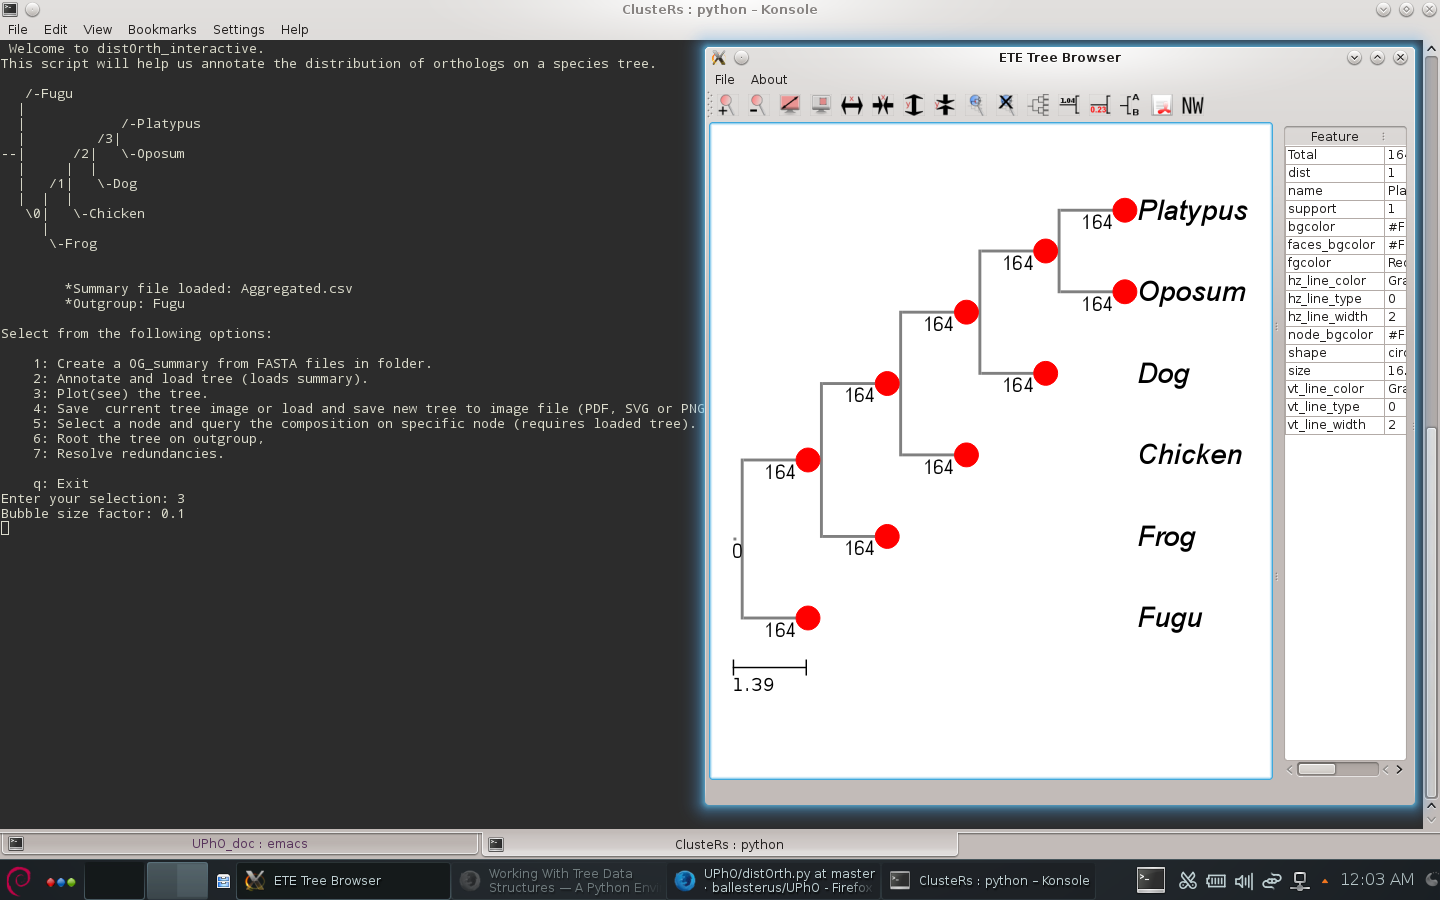
\includegraphics[width=\textwidth]{distOrthWithBub}
\caption{Screenshot with of distOrth\_interactive and the ETE2 tree on a example tree.}
\end{figure}

\subsection{Redundancies}
Depending on how the initial gene homologies were produced, the collection of orthogroups may not be mutually exclusive. From a biological perspective, some of these redundancies can be attributed to domain homologies, while others are artifacts of our clustering methods. Some orthogroups may be a subset of other ones (when all sequences are members in another)  and in cases with ambiguity in the orthology assessment one or more  sequences may be present  in orthogroups derived from the same gene-family.

The option number 7 in \texttt{distOrth\_interactive.py} remove such cases of sequence redundancy. The user is prompted to provide the name of the file to process,again a file in the \texttt{UPhO\_orthogroups.csv}. Next, the user chooses what type of redundancies should be resolved. In the case of removing subsets, the super-set orthogroup is retained. In the case of intersection form the same orthogroup, the largest one is preferred over the smaller ones. For each process cleaned text files are written (\texttt{OG\_no\_subsets.txt , OG\_no\_intersec.txt.}) along with ``log'' files reporting points of conflict and actions taken.

Finally, another type of redundancy, derived from different primary homologs may still exist in the dataset. A closer inspection is necessary to solve these cases as they are either product of domain specific homology or poor clustering performance. For phylogenomic analyses, clustering methods that produce mutually exclusive sets of homologs may be a better choice. 


\bibliography{references}

\end{document}